
\documentclass{beamer}

\usepackage{setspace}
\usepackage{varioref}

\newcommand{\q}[1]{{\fontfamily{phv}\selectfont ``}#1{\fontfamily{phv}\selectfont ''}} 


%%??\usepackage{spath3}
%\usepackage{pstricks}

\usepackage{amssymb}
\usepackage{textcomp}
\usepackage{tikz}

\newcommand{\colorbullet}[1]{{\color{#1}\ensuremath{\bullet}}}

%\usetikzlibrary{shapes,snakes}
%%?\usepackage[backslant]{aurical}

%%?\usepackage{hanging}

%\usepackage{DejaVuSerif}

\usepackage{setspace}

\usepackage[outline]{contour}



%{{\color{red!60!yellow}{\textbf{#1}}}}}}}

\usepackage{microtype}
\usepackage{hyphenat}
%%?\usepackage{dashrule}
%\usepackage[usenames,dvipsnames]{xcolor}

\usetikzlibrary{arrows, positioning, shapes}
\usetikzlibrary{backgrounds}


%%?\usepackage{wrapfig}

\usetikzlibrary{arrows, positioning, shapes}

%
%
%\usetheme{Singapore}

%\usetheme{AnnArbor}
%\usecolortheme{spruce}

\usetheme{BerkeleyAA}
\usecolortheme{spruceaa}

\def\swidth{1cm}
\setbeamersize{sidebar width left=\swidth}
%\addtobeamertemplate{frametitle}{\vspace*{6cm}}{\vspace*{0.3cm}}

\usepackage{mdframed}

\newcommand{\ft}[1]{\vspace*{.25cm}\raisebox{-.45cm}{%
\contour{MSUgreen!50!yellow}{{\protect\Huge{\protect\textbf{#1}}}}}}


%C:/dgch-dev/cpp/testdia/bulletin/reslides/beamerthemeBerkeley.sty
%:/dgch-dev/cpp/testdia/bulletin/reslides/beamerthemeAnnArbor.sty
%C:/dgch-dev/cpp/testdia/bulletin/reslides/beamerthemeAntibes.sty
%C:/dgch-dev/cpp/testdia/bulletin/reslides/beamerthemeBergen.sty

%\usecolortheme{frigatebird}
%\usecolortheme{spruce}
%
%\usetheme{Berlin}
%
%\usecolortheme{spruce}
%\usecolortheme{wolverine}

\setbeamertemplate{blocks}[rounded][shadow=true]
\setbeamertemplate{frametitle}[default][center]
\setbeamertemplate{caption}[numbered]

\setlength{\paperwidth}{10.in}
\setlength{\paperheight}{7.5in}
\setlength{\textwidth}{9.in}
\setlength{\textheight}{6.5in}

\newcommand{\curlyquote}[1]{{\fontfamily{gar}\selectfont{``}}#1%
{\fontfamily{gar}\selectfont{''}}}

\newcommand{\curlyapos}[1]{{\fontfamily{gar}\selectfont{'}}}

\newcommand{\cfbox}[2]{%
	\colorlet{currentcolor}{.}%
	{\color[rgb]{#1}%
		\fbox{\color{currentcolor}#2}}%
}


%%?\usecolortheme{spruce}

%\setbeamercolor{block title}{red}   
%\setbeamercolor{block title}{red}   

%%\usecolortheme{orchid}
%\usepackage{float}

%\setbeamerfont{itemize/enumerate body}{size=\small}
%\setbeamerfont{normaltext}{size=\}
%\setbeamerfont{block body}{size=\small}
\setbeamerfont{block title}{size=\large}
%\setbeamerfont{block body example}{size=\tiny}

\newcommand{\colortriangle}{{\color[rgb]{0.45, 0.4, 0.28}$\blacktriangleright$}}
	
\newcommand\FourQuad[4]{%
	
	\begin{minipage}[b][.45\textheight][t]{.47\textwidth}#1\end{minipage}\hfill%
	\begin{minipage}[b][.45\textheight][t]{.47\textwidth}#2\end{minipage}\\[0.5em]
	\begin{minipage}[b][.45\textheight][t]{.47\textwidth}#3\end{minipage}\hfill
	\begin{minipage}[b][.45\textheight][t]{.47\textwidth}#4\end{minipage}%
}

\newcommand\ThreeQuad[3]{%
	\hspace{2pt}\begin{minipage}[b][.23\textheight][c]{.99\textwidth}#1\end{minipage}\hfill%
	\begin{minipage}[b][.75\textheight][t]{.55\textwidth}#2\end{minipage}\hfill
	\begin{minipage}[b][.75\textheight][t]{.43\textwidth}#3\end{minipage}%
}

\newcommand\TwoQuad[2]{%
	\begin{minipage}[b][.75\textheight][t]{.55\textwidth}#1\end{minipage}\hfill
	\begin{minipage}[b][.75\textheight][t]{.43\textwidth}#2\end{minipage}%
}

\newcommand\OneQuad[1]{%
	\begin{minipage}[b][.45\textheight][t]{1.01\textwidth}#1\end{minipage}\hfill
	%\begin{minipage}[b][.75\textheight][t]{.43\textwidth}#2\end{minipage}%
}


\newenvironment{quadblock}[1]{\begin{block}{\begin{center}\Large{%
\colorbox[rgb]{0.25,0.1,0.25}{\color{yellow}{\textbf{#1}}}
}\end{center}}%
\begin{minipage}[c]{.97\textwidth}\vspace{1em}
}{
\end{minipage}
\end{block}}


\newenvironment{mpblock}[1]{\begin{block}{\begin{center}\Large{%
\colorbox[rgb]{0.25,0.1,0.25}{\color{yellow}{\textbf{#1}}}
}\end{center}}%
\begin{minipage}[c]{.97\textwidth}\vspace{1em}
\begin{textsf}}{\end{textsf}
\end{minipage}
\end{block}}

\usepackage{aurical}

%%?\usepackage{pbsi}
%\usepackage{oesch}
%\usepackage{LobsterTwo}

%\newcommand{\doubleCenteredFramebox}[1]{%
%\begin{center}%
%\framebox{%
%\begin{minipage}{0.85\textwidth}\begin{center}%
%#1\end{minipage}\end{center}}\end{center}}

%\setlength{\fboxsep}{0.15em}



\newcommand{\doubleCenteredFramebox}[1]{%
\setlength{\fboxsep}{2em}\setlength{\fboxrule}{2pt}
\begin{center}\cfbox{0.1, 0.5, 0.8}{\begin{minipage}{0.85\textwidth}\begin{center}\setlength{\fboxsep}{.25em}#1
	\end{center}\end{minipage}}\end{center}}


\newcommand{\halfPageFramebox}[1]{%
	\setlength{\fboxsep}{2em}\setlength{\fboxrule}{1pt}
	\begin{center}\cfbox{0.1, 0.5, 0.8}{\begin{minipage}{0.5\textwidth}\begin{center}\setlength{\fboxsep}{.25em}#1
				\end{center}\end{minipage}}\end{center}}

\newcommand{\sfitem}[1]{\item \LARGE{\textbf{\textsf{#1}}}}				

\renewcommand*\rmdefault{cmfib}

\newcommand{\scitem}[1]{\item {\Large{{\fontfamily{pag}\selectfont \textbf{#1}}}}}			
\newcommand{\smscitem}[1]{\item {\small{{\fontfamily{pag}\selectfont \textbf{#1}}}}}			


\newcommand{\embitem}[1]{\item \textbf{{\large #1}}}			


\newcommand{\highlightframebox}[1]{\cfbox{1,.5,1}{#1}}

%\begin{minipage}[.45\textheight][t]}{\end{minipage}\end{block}}

\newcommand{\manyasciimacron}{\textasciimacron\textasciimacron\textasciimacron%
\textasciimacron\textasciimacron\textasciimacron\textasciimacron\textasciimacron\textasciimacron%
\textasciimacron\textasciimacron\textasciimacron\textasciimacron\textasciimacron\textasciimacron%
\textasciimacron\textasciimacron\textasciimacron\textasciimacron\textasciimacron\textasciimacron%
}

\newcommand{\manyemdash}{\texttwelveudash\texttwelveudash\texttwelveudash\texttwelveudash\texttwelveudash%
 \texttwelveudash\texttwelveudash\texttwelveudash\texttwelveudash\texttwelveudash\texttwelveudash\texttwelveudash%
 \texttwelveudash\texttwelveudash\texttwelveudash\texttwelveudash\texttwelveudash\texttwelveudash\texttwelveudash%
}


\newenvironment{lightquadblock}[1]{\begin{center}\LARGE{%
			\colorbox[rgb]{.99,.99,0.66}{\color[rgb]{.14,.14,.04}{\hspace{-1em}\makebox[\textwidth]{#1}}}
		}\end{center}
		%\begin{framebox}
		\begin{minipage}[c]{.9\textwidth}\vspace{1em}
		}{
	\end{minipage}}
	
	
	\newenvironment{lightqblock}[1]{\begin{center}\LARGE{%
				\colorbox[rgb]{.90,.90,0.90}{\cfbox{.96,.94,.96}{\color[rgb]{.2,.06,.04}{\hspace{-1em}\makebox[\textwidth]{#1}}}}
			}\end{center}
			%\begin{framebox}
			\begin{minipage}[c]{.99\textwidth}\vspace{1em}
			}{
		\end{minipage}}
		

\newcommand\TwoQuadV[4]{%
	\begin{minipage}[b][.20\textheight][t]{1.04\textwidth}\begin{lightqblock}{#1}#2\end{lightqblock}\end{minipage}
	\begin{center}\begin{minipage}[t][.78\textheight][t]{.9\textwidth}%
		\begin{quadblock}{#3}\begin{minipage}{\textwidth}#4\end{minipage}\end{quadblock}\end{minipage}\end{center}%
}


%\newcommand{\conversationPatterns}{\framebox{%
%Conver\-\\
%sation\\
%Patterns}}

\newcommand{\reParser}{	
\begin{minipage}{32pt}\centering{\begin{scriptsize}\textbf{Relae\\\vspace{-6pt}Parser}\end{scriptsize}} 
\end{minipage}}

\usetikzlibrary{decorations.markings}
\usetikzlibrary{decorations.pathmorphing}

%\newcommand{\q}[1]{``#1"}

\definecolor{quadgrey}{rgb}{.9,.9.,.89}
\colorlet{snakegrey}{black!80!white}
\colorlet{blbl}{blue!20!black}

\definecolor{lqboutercolor}{rgb}{.92,.91,.93}
\definecolor{lqbinnercolor}{rgb}{.98,.98,.98}

\definecolor{blGreen}{rgb}{.2,.7,.3}
\definecolor{darkRed}{rgb}{.2,.0,.1}

\definecolor{postLinkColor}{rgb}{.5,.5,.1}

\definecolor{fcBoxColor}{rgb}{.8,.6,.3}

\definecolor{BlueGreen}{rgb}{.1,.6,.4}

\colorlet{ry}{red!80!yellow}
\colorlet{rblue}{red!70!blue}
\colorlet{rb}{rblue!40!black}
\colorlet{bg}{blGreen!40!black}

\newcommand{\hc}[1]{{\Huge %
{\contour{ry}{\protect\contour{rb}{{\protect\color{blGreen!40!black}{\protect\textbf{#1}}}}}}}}

\colorlet{yy}{yellow!80!blue}
\colorlet{yo}{yellow!80!orange}
\colorlet{yw}{yellow!20!white}



%\usepackage{microtype}



\newcommand{\yhc}[1]{{ %
{\contourlength{1.2pt}
{{\protect\contour{yw!50}{\protect\contour{yo!50}{{\protect\color{yy}{\protect\textbf{%
{\protect\Huge{\protect\textls[240]{#1}}}}}}}}}}}}}


\newcommand{\cframedbox}[1]{\begin{mdframed}
[linecolor=rb!85!red,linewidth=0.4mm]#1\end{mdframed}}

\newcommand{\cframedboxyellow}[1]{\begin{mdframed}
[linecolor=rb!45!yellow,linewidth=0.4mm]#1\end{mdframed}}

\newenvironment{postfragment}{\begin{minipage}{5.4cm}\begin{small}}
{\end{small}\end{minipage}}

\newenvironment{postComment}{\begin{minipage}{8cm}\begin{small}}
{\end{small}\end{minipage}}

\newenvironment{postLongComment}{\begin{minipage}{9cm}\begin{small}}
		{\end{small}\end{minipage}}


\newenvironment{tightcenter}{%
	\setlength\topsep{0pt}
	\setlength\parskip{0pt}
	\begin{center}
	}{%
\end{center}
}

\newcommand{\tightcenterline}[1]{\begin{tightcenter}#1\end{tightcenter}}



\definecolor{postBkgColor}{rgb}{.95,.85,.95}
\definecolor{postCommentBkgColor}{rgb}{.85,.85,.95}

\definecolor{grammarArrowColor}{rgb}{.85,.85,.45}

\tikzstyle{postStyle}=[draw=yellow!120,rounded corners,fill=postBkgColor,thin,inner sep=.2cm]
\tikzstyle{postCommentStyle}=[draw=postCommentBkgColor,double,fill=postCommentBkgColor,thick,inner sep=.2cm]

\tikzstyle{sdComponent}=[double,rounded corners,draw=brown!120,fill=blue!50,thin,inner sep=.2cm]
\tikzstyle{cnvComponent}=[double,shape=diamond,rounded corners,draw=brown!120,fill=blue!50,thin,inner sep=0cm]

\tikzstyle{baseStyle}=[fill=purple!50,draw=cyan!20,ultra thick,double,shape=diamond,inner sep=.15cm]
\tikzstyle{componentStyle}=[fill=red!50,draw,shape=ellipse,inner sep=.15cm]

\tikzstyle{componentExtendedStyle}=[fill={rgb:red,10;green,10;blue,2},draw,shape=rectangle,inner sep=.15cm]

\newcommand{\emphcolor}{%
	\colorlet{currentcolor}{.}%
	\color[rgb]{.4,.4,.4}}

\newcommand{\ncolor}{%
	\color{currentcolor}}


\definecolor{slidePartHeadColor}{rgb}{0,.2,.1}

\newcommand{\slidePartHead}[1]{{\fontfamily{pnc}\selectfont\color{slidePartHeadColor}\LARGE#1}}

\newcommand{\slidePartHeadCenter}[1]{\slidePartHead{\begin{minipage}{\textwidth}\begin{center}#1\end{center}\end{minipage}}}

\newcommand{\componentLabel}[1]{\begin{minipage}{3.5cm}\begin{center}#1\end{center}\end{minipage}}
\newcommand{\baseComponentLabel}[1]{\begin{minipage}{2cm}\textbf{\begin{center}#1\end{center}}\end{minipage}}

\newcommand{\componentExtendedLabel}[1]{\begin{minipage}{10cm}\begin{center}\textbf{#1}\end{center}\end{minipage}}

\newcommand{\cstd}[1]{\textbf{{\color[rgb]{.4,.4,.1}#1}}}

\usepackage{setspace}

%\fontfamily{pag}\selectfont \textbf{
\newcommand{\raiseBoxL}[1]{\makebox{\raisebox{.1em}{{\fontfamily{put}\fontseries{sb}\selectfont #1}\hspace{1.2em}}}}
%	\begin{textsf}{\small}{}\end{textsf}\end{minipage}}

\newcommand{\doubleFrame}[1]{%
\fcolorbox{fcBoxColor!90!cyan}{gray!50}{
%{\begin{center}
\begin{minipage}{.985\textwidth}
%\begin{center}	
\hspace{2pt}\vspace*{1pt}		
\fcolorbox{fcBoxColor!50!cyan}{white}{%
\begin{minipage}{.98\textwidth}%
\begin{center}\begin{minipage}{.955\textwidth}				
\begin{spacing}{1}\vspace{1em}\part{title}#1\end{spacing}%
\end{minipage}\end{center}
\end{minipage}}
%\end{center}
\end{minipage}}
%\end{center}}
}%

\usepackage{aurical}
\usepackage[T1]{fontenc}
\usepackage{libris}
\usepackage{relsize}

\newcommand{\VersatileUX}{{\color{red!85!black}\Fontauri Versatile}%
{{\fontfamily{qhv}\selectfont\smaller UX}}}


\newcommand{\doubleFrameTwo}[2]{%
\begin{center}
\begin{minipage}{\textwidth}	
\fcolorbox{fcBoxColor!50}{gray!50}{
%	\begin{center}
\begin{minipage}{\textwidth}
	\begin{center}
			%\hspace{4pt}\vspace*{2pt}		
			\fcolorbox{fcBoxColor!90}{white}{%
				\begin{minipage}{.95\textwidth}%
\begin{center}\begin{minipage}{.91\textwidth}#1\end{minipage}\end{center}%
				\end{minipage}}\vspace*{.5em}\\
%\vspace*{2pt}
%\hspace{4pt}				
\fcolorbox{fcBoxColor!90}{white}{
		\begin{minipage}{.94\textwidth}
\begin{center}\begin{minipage}{.91\textwidth}#2\end{minipage}\end{center}%
		\end{minipage}}
\end{center}		
\end{minipage}
%
}\par 
\end{minipage}
\end{center}		
}

\newcommand{\itup}[1]{\raisebox{2pt}{{\normalsize(#1)}}}

\newcommand{\FER}{{\color[rgb]{0.1,0.25,0.6}{FER}}}
\newcommand{\BER}{{\color[rgb]{0.1,0.25,0.6}{BER}}}
\newcommand{\IR}{{\color[rgb]{0.1,0.25,0.6}{IR}}}

\newcommand{\FrontEnd}{{\color[rgb]{0.1,0.25,0.6}{Front-End}}}
\newcommand{\BackEnd}{{\color[rgb]{0.1,0.25,0.6}{Back-End}}}
\newcommand{\Intermediate}{{\color[rgb]{0.1,0.25,0.6}{Intermediate}}}

%\newcommand{\doubleFrameTwo}[2]{%
%\fcolorbox{fcBoxColor}{gray!50}{
%\begin{minipage}{.98\textwidth}
%\hspace{4pt}\vspace*{2pt}	
%\fcolorbox{fcBoxColor}{white}{%
%\begin{minipage}{.95\textwidth}#1
%\end{minipage}}#1
%\fcolorbox{fcBoxColor}{white}{%
%\begin{minipage}{.95\textwidth}#2%
%\end{minipage}}
%}


%\newenvironment{doubleFrame}{%
%\fcolorbox{fcBoxColor}{gray!50}{\begin{minipage}{\textwidth}}
%{\end{minipage}}}

%\newenvironment{doubleFrame}{% \fcolorbox{fcBoxColor}{gray!50}{%
%\fbox{\begin{minipage}{\textwidth}%
%}
%{\end{minipage}}}
%}}
\usetikzlibrary{shadows}
\definecolor{logoRed}{rgb}{.3,0,0}
\definecolor{logoPeach}{RGB}{255, 159, 102}
\definecolor{logoCyan}{RGB}{66, 206, 244}
\definecolor{logoBlue}{RGB}{4, 2, 25}

\usepackage{changepage}

\newcommand{\nodeincludegraphicsLOCTRV}[7]{
\node[anchor=south west,inner sep=0,thick,
drop shadow={top color=logoBlue!50!logoCyan,
              bottom color=logoRed!50!logoCyan,
              shadow xshift=-1pt,
              shadow yshift=-3pt,
              rounded corners}] (image) at (#1){%
\fcolorbox{logoRed}{logoPeach!40!logoRed}{\includegraphics[scale=#2,trim={#5 #4 #3 #6},clip]{#7}}};}

%\newcommand{\doubleFrame}[1]
\newcommand{\nodeincludegraphics}[2][0.8\textwidth]{
\node[anchor=south west,inner sep=0] (image) at (0,0){%
\includegraphics[width=#1]{#2}};}

\newcommand{\nodeincludegraphicsR}[2][1]{
\node[anchor=south west,inner sep=0] (image) at (0,0){%
\includegraphics[scale=#1]{#2}};}

\newcommand{\nodeincludegraphicsAS}[1]{
\node[anchor=south west,inner sep=0] (image) at (0,0){%
\includegraphics{#1}};}

%\newcommand{\nodeincludegraphicsLOC}[3]{
%\node[anchor=south west,inner sep=0] (image) at (#1){%
%\includegraphics[scale=1]{#3}};}

\newcommand{\nodeincludegraphicsLOC}[3]{
\node[anchor=south west,inner sep=0] (image) at (#1){%
\includegraphics[scale=#2]{#3}};}

\newcommand{\nodeincludegraphicsTRRSqqq}[6]{
\node[anchor=south west,inner sep=0] (image) at (0,0){%
\includegraphics[scale=#1,trim={#2 #3 #4 #5},clip]{#6}};}

\newcommand{\nodeincludegraphicsTR}[3]{
\node[anchor=south west,inner sep=0] (image) at (0,0){%
\includegraphics[trim={0 #2 #1 0},clip]{#3}};}

\newcommand{\nodeincludegraphicsTRR}[5]{
	\node[anchor=south west,inner sep=0] (image) at (0,0){%
		\includegraphics[trim={#3 #2 #1 #4},clip]{#5}};}

\newcommand{\nodeincludegraphicsTRRS}[6]{
\node[anchor=south west,inner sep=0,scale=#1] (image) at (0,0){%
\includegraphics[trim={#4 #3 #2 #5},clip]{#6}};}


\newcommand{\ann}[9]{%
	\path [draw=#1,draw opacity=#2,line width=#3, fill=#4, fill opacity = #5, even odd rule] %
	(#6) ellipse(#7 and #8) ellipse(#7*#9 and #8*#9);}

\newcommand{\polyann}[9]{%
\path [draw=#1,draw opacity=#2,line width=#3, fill=#4, fill opacity = #5, even odd rule] %
	node [minimum size=#8,regular polygon,regular polygon sides=#7] at (#6) {}
	node [minimum size=#9,regular polygon,regular polygon sides=#7] at (#6) {};}
	

%\newcommand{\polyann}[9]{%
%	\path [draw=#1,draw opacity=#2,line width=#3, fill=#4, fill opacity = #5, even odd rule] %
%	path minimum size=2cm,regular polygon,regular polygon sides=6(#7 and #8) ellipse(#7*#9 and %#8*#9);}


\makeatletter
\newcommand*\getX[1]{\expandafter\getX@i#1\@nil}
\newcommand*\getY[1]{\expandafter\getY@i#1\@nil}
\def\getX@i#1,#2\@nil{#1}
\def\getY@i#1,#2\@nil{#2}
\makeatother

\newcommand{\rectann}[9]{%
	\path [draw=#1,draw opacity=#2,line width=#3, fill=#4, fill opacity = #5, even odd rule] %
	(#6) rectangle(\getX{#6}+#7,\getY{#6}+#8)
	({\getX{#6}+((#7-(#7*#9))/2)},{\getY{#6}+((#8-(#8*#9))/2)}) rectangle %
	({\getX{#6}+((#7-(#7*#9))/2)+#7*#9},{\getY{#6}+((#8-(#8*#9))/2)+#8*#9});}

\newcommand{\rectanneatdbl}[9]{%
	\path [draw=#1,draw opacity=#2,line width=#3, fill=#4, fill opacity = #5, even odd rule] %
	(#6) rectangle(\getX{#6}+#7,\getY{#6}+#8)
	({\getX{#6}+\getX{#9}},{\getY{#6}+\getY{#9}}) rectangle %
	({\getX{#6}+#7-\getX{#9}},{\getY{#6}+#8-\getY{#9}})
	;}

\newcommand{\rectanneat}[9]{%
	\path [draw=#1,draw opacity=#2,line width=#3, fill=#4, fill opacity = #5, even odd rule] %
	(#6) rectangle(\getX{#6}+#7,\getY{#6}+#8)
	({\getX{#6}+(#7/abs(#7))*#9},{\getY{#6}+(#8/abs(#8))*#9})
	rectangle({\getX{#6}+#7-(#7/abs(#7))*#9},{\getY{#6}+#8-(#8/abs(#8))*#9});}

\newcommand{\colorarr}[8]{
	\draw [#1, draw=#2,draw opacity=#3,
	fill=#4,fill opacity=#5,line width=#6] (#7) to (#8);
}

\colorlet{brred}{brown!53!red}
\colorlet{grred}{grammarArrowColor!40!red!60}

\definecolor{elColor}{rgb}{.2,.1,0}
\definecolor{flColor}{rgb}{0.7,0.3,0.3}

\definecolor{logoOrange}{RGB}{108, 18, 30}
\definecolor{logoGreen}{RGB}{85, 153, 89}
\definecolor{logoPurple}{RGB}{200, 208, 30}

\definecolor{logoBlue}{RGB}{4, 2, 25}
\definecolor{logoPeach}{RGB}{255, 159, 102}
\definecolor{logoCyan}{RGB}{66, 206, 244}
\definecolor{logoRed}{rgb}{.3,0,0}



\newcommand*{\MyDiamond}{%
	\begin{tikzpicture}{baseline}	
	\node [draw, shape=diamond, %shape border rotate=100,
	line width=.2mm, left color=flColor, right color=darkRed, draw=logoPurple, aspect=1,
	draw opacity=0.6, fill opacity=0.8, xscale=0.5, yscale=0.5,
	minimum width=1mm, 
	] 
	at (2, 0) {};\end{tikzpicture}}


\newcommand{\nodeincludegraphicsLOCTR}[7]{
\node[anchor=south west,inner sep=0,thick,
drop shadow={top color=logoBlue!50!logoCyan,
              bottom color=logoRed!50!logoCyan,
              shadow xshift=-1pt,
              shadow yshift=-3pt,
              rounded corners}] (image) at (#1){%
\fcolorbox{logoRed}{logoPeach!40!logoRed}{\includegraphics[scale=#2,trim={#5 #4 #3 #6},clip]{#7}}};}



\begin{document}

%\input{cqlDescriptionSlide}

\atsp
\begin{frame}{\parbox{20cm}{\centering\ft{Dataset Creator}\\ 
%\ft{\fontsize{23}{22}\selectfont Integrated with Cloud Back-Ends}\\ 
\ft{\LARGE{(\curlyquote{dsC})}}}}
\section{Intro}
\vspace{-2em}

%\colorbox{cyan}{
%\begin{minipage}{.43\textwidth}
%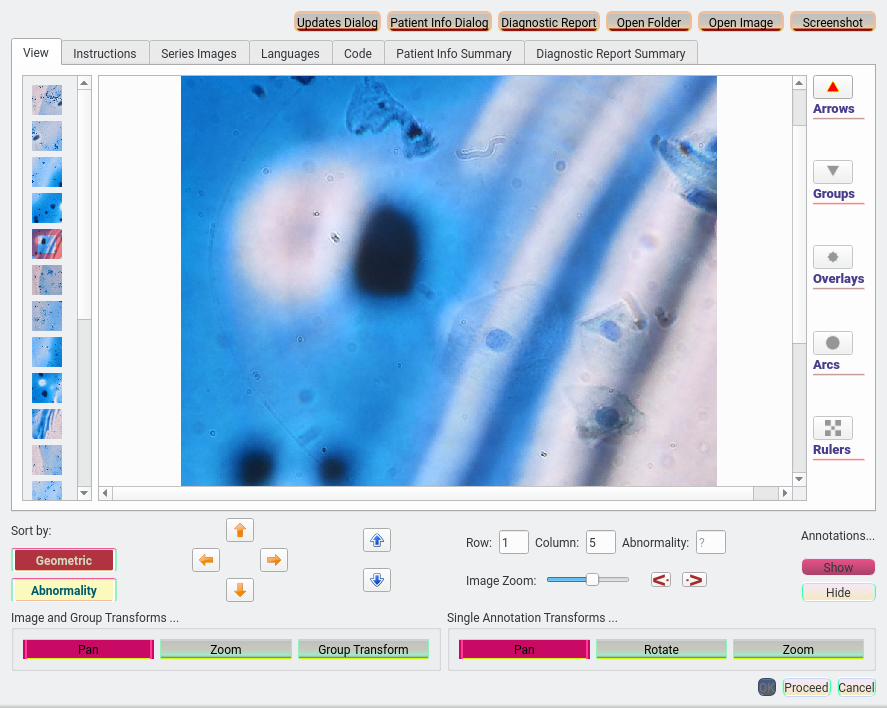
\includegraphics[scale=.5]{slide1pic1.png}
%\end{minipage}\begin{minipage}{.5\textwidth}
%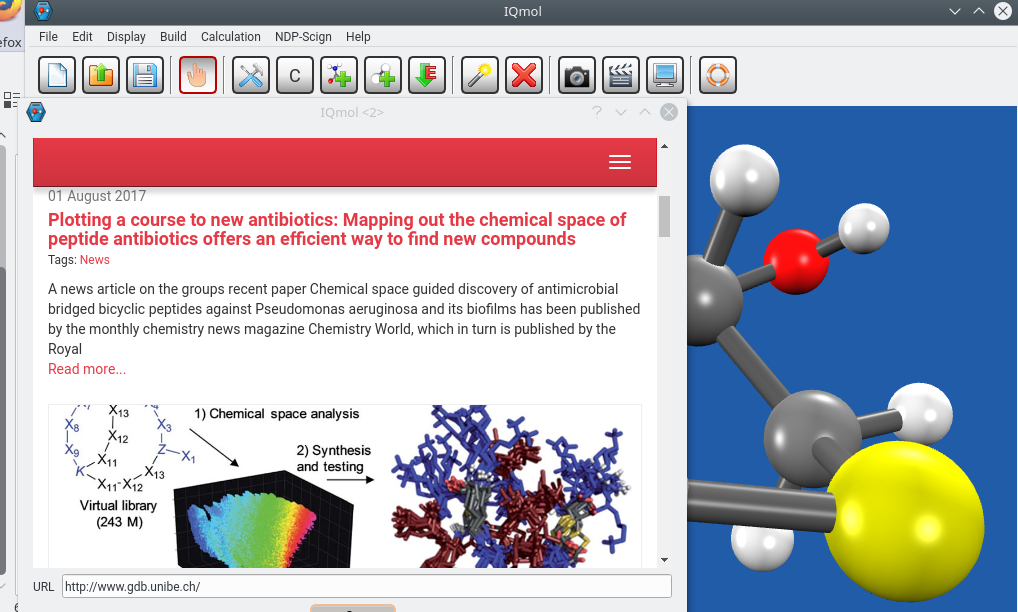
\includegraphics[scale=.5]{slide1pic1a.png}
%\end{minipage} }

\definecolor{pd}{RGB}{200,60,30}

%\begin{adjustwidth*}{-2em}{} 
\hspace*{10pt}\begin{tikzpicture}

%\node [fill=white] at (20,0) {PITCH DECK};


\nodeincludegraphicsLOCTR{13.6,3.7}{0.35}{4cm}{0cm}{1cm}{0cm}{after/slide1pic1a.png}

\nodeincludegraphicsLOCTR{17,0.1}{0.3}{0cm}{0cm}{0cm}{0cm}{after/Pub-4.png}


\nodeincludegraphicsLOCTR{0,0}{0.64}{1.2cm}{4cm}{1cm}{1cm}{after/slide1pic1.png}

\end{tikzpicture}
%\end{adjustwidth*}



\vspace{.5em}
		
%\hspace{2m}
\colorbox{white}
{%
\setlength{\fboxsep}{0pt}{\parbox{\textwidth}{%			
\begin{center}
\colorbox[RGB]{200,60,30}	
{\setlength{\fboxsep}{8pt}				
\hspace{3pt}\colorbox{white}{\setlength{\fboxsep}{0pt}
%\framebox{
\LARGE\begin{minipage}{.85\textwidth}
\vspace{4pt}\centering
Linguistic Technology Systems (LTS) \\
Amy Neustein, Ph.D., Founder and CEO \\
amy.neustein@verizon.net \\
(917) 817-2184 
\end{minipage}
%}
}
\hspace{1pt}
}
\end{center}
}}
}
\end{frame}


\begin{frame}{\ft{Our NCN (Native Cloud/Native) Protocol for Cloud Backends}}
	\section{NCN}
\vspace{-3em}	
{\Large\fontfamily{uhv}\selectfont
\vspace{1em}
\begin{center}
\begin{minipage}{.9\textwidth}
\vspace{1em}
\fcolorbox{lqboutercolor}{lqbinnercolor}{\begin{minipage}{\textwidth}%
\begin{lightquadblock}{Cloud/Native Components as Back-Ends 
for Native Software}
\begin{center}\begin{minipage}{.99\textwidth}
{\Large \begin{itemize}
\sqitem {\lsep} \parbox[t]{17cm}{Our \q{Native Cloud/Native} service is a protocol, which refers to native application front-ends paired with 
Cloud/Native (back-end) container instances.}\vspace{1em}
\sqitem {\lsep}  Code libraries and data representation may be shared 
across both endpoints.\vspace{1em}
\sqitem {\lsep}  \parbox[t]{17cm}{Common representation on both server- and client-side 
streamlines network communications (no need to marshal data between 
different formats).}\vspace{1em}
\sqitem {\lsep}  \parbox[t]{17cm}{Our NCN technology 
can be ported to other (non-Qt) application frameworks 
(wxWidgets, XCode, MFC, etc.).\\
\hspace*{5pt}{\MyOct}\hspace{-4pt} Note: This presentation will focus on NCN's default 
Qt{} implementation.} 
\\\vspace{1em}
\end{itemize}}\end{minipage}
\end{center}
\end{lightquadblock}
\end{minipage}}
\fcolorbox{lqboutercolor}{lqbinnercolor}{\begin{minipage}{\textwidth}%
\begin{lightquadblock}{How Cloud Back-Ends Enhance Native Front Ends}
{\Large\begin{itemize}
\sqitem {\lsep}  Cloud Backup {\MyOct} Share Data between Users {\MyOct} Collaborative Editing \vspace{1em}
\sqitem {\lsep}  \parbox[t]{14cm}{Maintain users' application state across different 
computers (home/school/office)\vspace{1em}}
\sqitem {\lsep}  Upgrade running applications without needing to re-compile
\vspace{1em}
\end{itemize} }
\end{lightquadblock}
\end{minipage}}

\end{minipage}
\end{center}
}

\end{frame}


\begin{frame}{\ft{Application-As-A-Resource (A3R)}}
\vspace{.5em}	

%{\begin{minipage}[c]{\textwidth}\Large\centering\color{slidePartHeadColor} 	
%{\color[rgb]{.3,.1,0}{\Huge\fontfamily{bch}\fontseries{eb}\selectfont The A3R Protocol 
%Describes Applications as Self-Contained, Downloadable Code Resources}}\\
%\vspace{1em}	
%Combining Natural Language Processing and Conversation Analysis: \\
%for Next Generation Language and Conversation Tools\end{minipage}}
%\vspace{1em}
	
{\Large\fontfamily{uhv}\selectfont
\begin{minipage}{\textwidth}
\fcolorbox{fcBoxColor!50}{gray!50}{
\begin{minipage}{.98\textwidth}
\hspace{9pt}\vspace*{2pt}		
\fcolorbox{fcBoxColor}{white}{\begin{minipage}{.95\textwidth}%
\vspace{.8em}
{\centerline{\LARGE\color{darkRed} The A3R Application Model}}
\vspace{1em}\begin{itemize}
\item A3R Applications 	
\vspace{.3em}
\item A3R Applications		
\end{itemize}\vspace{.2em}
\end{minipage}}\\
\vspace*{1em}
\hspace{5pt}\fcolorbox{fcBoxColor}{white}{\begin{minipage}{.95\textwidth}%
\vspace{.8em}
{\centerline{\LARGE\color{darkRed} A3R Developer Tools}\vspace{.8em}}
\begin{itemize}
 \item Hypergraph-based data modling and serialization.
\vspace{.5em}  
 \item Framework for building custom scripting, parsing, and data persistence engines.
\vspace{.5em}   
 \item Enhanced support for applications specifically designed to access research data 
sets. 
 \end{itemize}\end{minipage}}\end{minipage}}
\end{minipage}}
\end{frame}


\begin{frame}{\ft{The Qt Ecosystem and the 
			Limitations of Qt in the Cloud}}
\section{Qt}
\vspace{.5em}	

{\begin{minipage}[c]{\textwidth}\Large\centering\color{slidePartHeadColor} 	
{\color[rgb]{.3,.1,0}{\Huge\fontfamily{bch}\fontseries{eb}\selectfont Qt is 
the most popular native, cross-platform application-development framework.}}\\
\vspace{1em}	
{\LARGE \MyDiamond{} \texttildelow{}1 million active developers \MyDiamond{}  Over 5,000 client companies \MyDiamond{}  
Worldwide \\\q{Qt Partners} Ecosystem  
\MyDiamond{} \texttildelow{}US \$25 billion overall market }\end{minipage}}
\vspace{1em}
	
{\Large\fontfamily{uhv}\selectfont
\vspace{1em}
\begin{center}
\begin{minipage}{.9\textwidth}
\vspace{1em}
\fcolorbox{lqboutercolor}{lqbinnercolor}{\begin{minipage}{\textwidth}%
\begin{lightquadblock}{However ... Limited Qt Cloud Integration Support}
\begin{center}\begin{minipage}{.98\textwidth}
{\LARGE \setlength{\leftmargini}{30pt}\begin{itemize}
\sqitem \hspace{.3em} \q{Qt Cloud Services} Discontinued in 2016. \vspace{1em}
\sqitem \hspace{.3em} \parbox[t]{14cm}{Currently there is no standard model for accessing 
\\Cloud services from Qt applications.}\vspace{1em}
\sqitem \hspace{.3em} \parbox[t]{14cm}{Nor is there a standard Qt-based Cloud/Native \\container architecture.}
\\\vspace{1.5em}
\end{itemize}}\end{minipage}
\end{center}
\end{lightquadblock}
\end{minipage}}


\end{minipage}
\end{center}
}

\end{frame}


\begin{frame}{\ft{Example Use-Cases}}
\vspace{-3em}	
{\Large\fontfamily{uhv}\selectfont
\vspace{1em}
\begin{center}
\begin{minipage}{.9\textwidth}
\vspace{1em}
\fcolorbox{lqboutercolor}{lqbinnercolor}{\begin{minipage}{\textwidth}%
\begin{lightquadblock}{Inter-Application Networking and Workflow Management}
\begin{center}\begin{minipage}{.98\textwidth}
{\bf \begin{itemize}
\item Export data and instructions between Qt-based applications (slides 6-7).\vspace{1em}
\item Embed document or multi-media viewers inside scientific or 
dataset applications (slides 18-21).\\\vspace{1.5em}
\end{itemize}}\end{minipage}
\end{center}
\end{lightquadblock}
\end{minipage}}
\fcolorbox{lqboutercolor}{lqbinnercolor}{\begin{minipage}{\textwidth}%
\begin{lightquadblock}{Responsive, desktop-style applications for enhanced UX}
\begin{itemize}
\item  Compelling front-ends for e-commerce, Real Estate, VR, etc. (slides 11-17).\vspace{1em}
\item  Native applications offer superior User Experience, leveraging distinct interactive 
features of desktop GUIs: context menus, 
dialog boxes, tool tips, Multiple Window Display, 
dock windows, etc. \vspace{1em}
\item  For scientists and researchers, 
build innovative data-collection instruments 
as well as interactive Research Object applications 
(slides 8-10).
\end{itemize} 
\end{lightquadblock}
\end{minipage}}

\end{minipage}
\end{center}
}

\end{frame}


%

\begin{frame}{\ft{EC-1}}

\doubleFrame{EC1.}

\begin{tikzpicture}
\nodeincludegraphicsTR{2.7cm}{2cm}{pics/RAD-1.png}

 \node [anchor=west,fill=brown!20!white,inner sep=7, text width=14cm]
  (longnote) at (5.5,7) {%  %{\color{rb!85!red}{
  {\cframedbox{\large \textbf{EC1}}}};

\end{tikzpicture}


\end{frame}




\begin{frame}{\ft{An Example of Inter-Application Networking}}

\doubleFrame{This slide and the next demonstrates a case-study 
where inter-application data sharing enhances two applications' capabilities --- 3DimViewer, a radiology tool, and MeshLab, a 3D graphics engine.}

\begin{tikzpicture}
\nodeincludegraphicsTR{2.7cm}{2cm}{pics/RAD-2.png}

 \node [anchor=west,fill=brown!20!white,inner sep=7, text width=14cm]
  (longnote) at (5.5,7) {\vspace{-8pt}%  %{\color{rb!85!red}{
  {\cframedbox{\large \textbf{3DimViewer builds 3D models from 
2D radiology image series ...}}}};

\end{tikzpicture}


\end{frame}




\begin{frame}{\ft{3D Graphics Sent to MeshLab}}

\doubleFrame{... Once the 3D tissue sample is constructed by 3DimViewer's algorithms, 
an A3R inter-application networking protocol (implemented 
as an extension to both components) allows 3DimViewer to 
export the model to MeshLab so that it may be studied in a 
more comprehensive 3D viewing environment.}

\begin{tikzpicture}
\nodeincludegraphicsTR{2.7cm}{2cm}{pics/RAD-3.png}

% \node [anchor=west,fill=brown!20!white,inner sep=7, text width=14cm]
%  (longnote) at (5.5,7) {%  %{\color{rb!85!red}{
%  {\cframedbox{\large \textbf{EC3}}}};

\end{tikzpicture}


\end{frame}





\begin{frame}{\ft{A3R Applications as Data Collection Instruments}}

%\doubleFrame{In medicine and social science, \q{data collection instruments} 
%(DCIs) refer to surveys, questionnaires, and other tools to get human feedback.}

\begin{tikzpicture}
\nodeincludegraphicsTRRS{1}{0cm}{0cm}{0cm}{0cm}{pics/Res-2a.jpeg}

 \node [anchor=west,inner sep=15, text width=5cm,top color=blue!20,
 bottom color=blue!40,
 rounded corners=6pt%,
 %blur shadow={shadow blur steps=2}
 ]
  (longnote) at (15.5,8) {\baselineskip=22pt%  %{\color{rb!85!red}{
  {\LARGE \textbf{In medicine and social science, \q{data collection instruments} 
  			(DCIs) refers to surveys, questionnaires, and other tools to get human feedback.}}\par};

\end{tikzpicture}


\end{frame}




\begin{frame}{\ft{Qt-Based Interactive Forms}}
\section{Research Slide 4}
\doubleFrame{Data Collection Instruments implemented as native desktop applications 
can have easily navigable, interactive forms that make it 
simpler for people to provide information ...}
\begin{tikzpicture}
\nodeincludegraphicsTR{2.7cm}{2cm}{pics/Res-1.jpeg}

\node at (4.9,13.65){};

 \node [anchor=west,inner sep=4, 
 top color=rb!85!yellow,
 %middle color=blue!40!black,
 bottom color=blue!40,
 rounded corners=1pt, text width=12cm]
  (longnote) at (5.72,12.72) {\vspace{-12pt}%  %{\color{rb!85!red}{
  {\cframedboxx{3pt}{3pt}{\Large \textbf{... Also, submitted information is 
already in digital form, eliminating the need for separate data entry.}}}};

\end{tikzpicture}


\end{frame}




\begin{frame}{\ft{A3R Applications as Research Objects}}
\section{Research Slide 5}
\doubleFrame{Complementary to A3R components
which facilitate \textit{obtaining} research 
or experimental data, A3R \q{Data-Set Applications} are also 
powerful tools for visualizing and analyzing research findings.}

\begin{tikzpicture}
\nodeincludegraphicsTRRS{0.92}{0cm}{0cm}{0cm}{0.8cm}{pics/Res-4.png}

 \node [anchor=west,bottom color=brown!90!red,top color=blue!40, inner sep=3, text width=16.5cm]
  (longnote) at (2.6,13.3) {\vspace{-8pt} %  %{\color{rb!85!red}{
  {\cframedboxx{0.7mm}{2pt}{\large \textbf{Data-Set Applications are \q{Research Object Bundles} --- combinations of code and data, 
providing access to data sets without the need for external software dependencies.\vspace{-2pt}}}}};

\end{tikzpicture}


\end{frame}





\begin{frame}{\ft{Native Applications as Interactive Catalogs}}
\section{E-Commerce Slide 1}
\doubleFrameX{0.983\textwidth}{As a case-study in enhanced User Experience afforded 
by native applications, consider how static PDF catalogs and 
brochures can be turbo-charged to engaging, interactive software-based 
\makebox{presentations}.}

\begin{tikzpicture}
\nodeincludegraphicsTRRS{0.84}{0cm}{1.5cm}{0.8cm}{0cm}{pics/EC-1.png}

% \node [anchor=west,fill=brown!20!white,inner sep=7, text width=14cm]
%  (longnote) at (5.5,7) {%  %{\color{rb!85!red}{
%  {\cframedbox{\large \textbf{EC1}}}};

\end{tikzpicture}


\end{frame}




\begin{frame}{\ft{Interactive \q{Shopping Carts}}}

\doubleFrame{Instead of static lists, shopping carts in a 
native context can be multi-scale, multi-window interactive displays.}

\begin{tikzpicture}
\nodeincludegraphicsTR{2.7cm}{2cm}{pics/EC-4.png}

% \node [anchor=west,fill=brown!20!white,inner sep=7, text width=14cm]
%  (longnote) at (5.5,7) {%  %{\color{rb!85!red}{
%  {\cframedbox{\large \textbf{EC2}}}};

\end{tikzpicture}


\end{frame}




\begin{frame}{\ft{Explore Products with Native Software}}

\doubleFrame{Interactive catalogs allow designers to incorporate 
many unique features and capabilities of desktop applications, 
such as using HSV color-wheel controls to explore color coordination 
while shopping.}

\begin{tikzpicture}
\nodeincludegraphicsTRRS{0.8}{1cm}{2.7cm}{0cm}{0}{pics/EC-3.png}

% \node [anchor=west,fill=brown!20!white,inner sep=7, text width=14cm]
%  (longnote) at (5.5,7) {%  %{\color{rb!85!red}{
%  {\cframedbox{\large \textbf{EC3}}}};

\end{tikzpicture}


\end{frame}


%

\begin{frame}{\ft{EC-4}}

\doubleFrame{EC4.}

\begin{tikzpicture}
\nodeincludegraphicsTR{2.7cm}{2cm}{pics/EC-4.jpg}

 \node [anchor=west,fill=brown!20!white,inner sep=7, text width=14cm]
  (longnote) at (5.5,7) {%  %{\color{rb!85!red}{
  {\cframedbox{\large \textbf{EC4}}}};

\end{tikzpicture}


\end{frame}





\begin{frame}{\ft{Interactive Real Estate}}
\section{E-Commerce Slide 4}
\doubleFrameY{1.01\textwidth}{-10pt}{1.005\textwidth}{\textwidth}{4pt}{A3R programming can also bring enhanced UX 
to Real Estate presentations --- instead of just groups of 
photos, properties may be displayed via interactive, multidimensionally-organized,
color-coded photo viewers.}

\begin{tikzpicture}
%\nodeincludegraphics[0.9\textwidth]{screenshots/ss-ph2.png}
\nodeincludegraphicsTRRS{1}{4.6cm}{2.2cm}{0.8cm}{1cm}{screenshots/ss-ph2.png}

\rectann{darkRed}{0.7}{1mm}{grammarArrowColor}{0.5}{0.05,0.5}{9.4}{5.25}{0.9}

\node [anchor=west,fill=brown!8!white,inner sep=12, 
opacity=0.88, text opacity=1] (note) at (15,3.89) {\hc{Current Photo}};

\colorarr{>=latex, ->}{fcBoxColor!60!black}
{0.8}{blGreen!30!red}{1}{1mm}{note.west}{6.58, 7.25}

\node [anchor=west,fill=brown!8!white,inner sep=12, 
opacity=0.88, text opacity=1] (note) at (11,2.29) {\hc{Color-Coded Groups}};

\colorarr{>=latex, ->}{fcBoxColor!60!black}
{0.8}{blGreen!30!red}{1}{1mm}{note.west}{9.58, 3.25}


\end{tikzpicture}


\end{frame}




\begin{frame}{\ft{Photo Viewer Interactive Cues}}

\doubleFrame{These slides demonstrate 
visual cues to aid photo navigation, 
such as color bands that switch from horizontal 
to vertical indicating which photos have been viewed; and the 
thumbnail of the current viewed photo 
marked with a thick colored border (this border will 
surround the thumbnail and both horizontal and 
vertical overlays).}

\begin{tikzpicture}
%\nodeincludegraphics[0.9\textwidth]{screenshots/ss-ph3.png}
\nodeincludegraphicsTR{5.5cm}{3.23cm}{screenshots/ss-ph3.png}

 %%\node [anchor=west] (note) at (11,11.2) {\Huge {\color{blGreen!30!black}Already Viewed}};

\node [anchor=west,fill=brown!8!white,inner sep=12, 
opacity=0.88, text opacity=1] (note) at (7,11.8) {\hc{Already Viewed (vertical color band)}};


%\ann{BlueGreen!30!red}{1}{.8mm}{blue!50!orange}{0.5}{3.61,8.95}{.4}{.6}{0.7}

\colorarr{>=latex, ->}{fcBoxColor!20!black}
{0.8}{darkRed!70!blue}{2}{1mm}{note.west}{3.7, 9}


\node [anchor=west,fill=brown!8!white,inner sep=12, 
opacity=0.88, text opacity=1] (note) at (6.3,9.7) {\hc{Not Yet Viewed (horizontal color band)}};

%\ann{BlueGreen!30!red}{1}{.8mm}{blue!50!orange}{0.5}{7.6, 7.3}{.73}{.35}{0.7}

%
\colorarr{>=latex, ->}{fcBoxColor!20!black}
{0.8}{darkRed!70!blue}{2}{1mm}{note.south}{8.2, 7.25}

%\node [anchor=west] (note) at (11,3) {\Huge {\color{blGreen!30!black}Current Photo}};

\node [anchor=west,fill=brown!8!white,inner sep=12, 
opacity=0.88, text opacity=1] (note) at (5,1.89) {\hc{Current Photo (viewed for the second time)}};

\colorarr{>=latex, ->}{fcBoxColor!60!black}
{0.8}{blGreen!30!red}{1}{1mm}{note.north west}{4.39, 4.75}


\end{tikzpicture}


\end{frame}




\begin{frame}{\ft{Filtering Photos}}
\section{E-Commerce Slide 6}
\doubleFrame{Another feature which may be conveniently 
implemented in \AtR{}-style photo viewers is a filtering 
option, which --- given a collection of pictures 
classified into several groups --- allows users 
to show or hide photos based on the group they belong to (note the check-box buttons on the group listing).}

\begin{tikzpicture}

\nodeincludegraphicsTRRS{1}{4cm}{0.05cm}{3cm}{1.35cm}{screenshots/ss-ph4.png}


\node [anchor=west,fill=brown!8!white,inner sep=12, 
opacity=0.88, text opacity=1] (note) at (4.5,8.2) {\hc{Visible Groups}};


\ann{BlueGreen}{1}{.8mm}{grammarArrowColor}{0.5}{3.61,5.5}{2.4}{.6}{0.7}
%\ann{BlueGreen!30!red}{1}{.8mm}{blue!50!orange}{0.5}{3.61,5.5}{2.4}{.6}{0.7}

%{BlueGreen}{0.3}{1mm}{grammarArrowColor}{0.5}

\colorarr{>=latex, ->}{fcBoxColor!60!black}
{0.8}{blGreen!30!red}{2}{1mm}{note.south}{6, 5.9}



\node [anchor=west,fill=brown!8!white,inner sep=12, 
opacity=0.88, text opacity=1] (cb) at (6,4.2) {\hc{Check Boxes}};

\draw[>=stealth, ->>,bend right=5, 
draw=orange!40!red,% rgb{0.5,0.1,0.4}, 
draw opacity=0.3,
fill=red!20!black, fill opacity=1, 
line width=1.2mm
] (cb.west) to (1.55, 3.61);


\node [anchor=west,fill=brown!8!white,inner sep=12, 
opacity=0.88, text opacity=1] (note) at (11,2.6) {\hc{Hidden Groups}};


\ann{BlueGreen!30!red}{1}{.8mm}{blue!50!orange}{0.5}{3.61,1.7}{2.4}{.6}{0.7}

\colorarr{>=latex, ->}{fcBoxColor!20!black}
{0.8}{darkRed!70!blue}{2}{1mm}{note.west}{6, 1.9}


%\node [anchor=west,fill=brown!8!white,inner sep=12, 
%opacity=0.88, text opacity=1] (note) at (6.7,9.7) {\hc{Not Yet Viewed (horizontal color band)}};

%\ann{BlueGreen!30!red}{1}{.8mm}{blue!50!orange}{0.5}{7.6, 7.3}{.73}{.35}{0.7}

%\colorarr{>=latex, ->}{fcBoxColor!20!black}
%{0.8}{darkRed!70!blue}{2}{1mm}{note.south}{8.2, 7.25}



%\node [anchor=west,fill=brown!8!white,inner sep=12, 
%opacity=0.88, text opacity=1] (note) at (5,1.89) {\hc{Current Photo (viewed for the second time)}};

%\colorarr{>=latex, ->}{fcBoxColor!60!black}
%{0.8}{blGreen!30!red}{1}{1mm}{note.north west}{4.35, 4.75}


\end{tikzpicture}


\end{frame}





\begin{frame}{\ft{Interactive VR: Hyperlinked Tag Posts}}

\doubleFrame{Panorama-Photography-based VR engines, 
like Materport, allow \q{tag posts} with embedded 
hyperlinks, which in a native-application 
context become 
channels of communication between the VR 
renderer  
and the host application.}

\begin{tikzpicture}
\nodeincludegraphicsTR{2.7cm}{2.4cm}{screenshots/ss-vt5.png}

\ann{darkRed}{0.7}{1mm}{grammarArrowColor}{0.5}{13,7}{5.5}{2}{0.9}

\node [anchor=west,fill=white,inner sep=11]
%(note) at (13,10) {\Huge {\color{blGreen!30!black}Hyperlinked Tag Posts}};
 (note) at (12,10) {\hc{Hyperlinked Tag Posts}};

\colorarr{>=latex, ->}{blGreen!80!blue}{0.7}
{cyan!60!red}{1}{2mm}{note.south}{15,6.5}


\end{tikzpicture}


\end{frame}





\begin{frame}{\ft{A3R Document Viewers}}
\section{Publishing Slide 1}
\doubleFrame{A3R applications may embed viewers for 
%popular 
document formats such as e-Pub, HTML, and PDF; 
 %The application may 
then supplement conventional publications 
with special components 
%software %components, perhaps 
customized for 
individual manuscripts --- here, a widget 
allowing readers to visually explore patterns in 
classical Indian music.}

\begin{tikzpicture}
\nodeincludegraphicsTRRS{0.95}{2cm}{3cm}{5cm}{.5cm}{pics/Pub-2.png}

% \node [anchor=west,fill=brown!20!white,inner sep=7, text width=14cm]
%  (longnote) at (5.5,7) {%  %{\color{rb!85!red}{
%  {\cframedbox{\large \textbf{EC1}}}};

\end{tikzpicture}


\end{frame}


\atsp
\begin{frame}{\ft{\AtR{} Document Viewers as Embedded Components}}
\section{Publishing Slide 2}
\doubleFrameY{\textwidth}{-7.5pt}{1.006\textwidth}{0.96\textwidth}{1pt}{%
Document Viewers may also be embedded in 
host applications which provide domain-specific 
\makebox{visualization} capabilities.  For example, chemistry papers 
might be viewed within IQmol (a Qt-based program for molecular visualization and physical/chemical analysis) via an \AtR{} document-viewer plugin.}

\begin{tikzpicture}
\nodeincludegraphicsTRRS{.8}{2cm}{2.7cm}{2cm}{0}{pics/Pub-1.png}

% \node [anchor=west,fill=brown!20!white,inner sep=7, text width=14cm]
%  (longnote) at (5.5,7) {%  %{\color{rb!85!red}{
%  {\cframedbox{\large \textbf{EC2}}}};

\end{tikzpicture}


\end{frame}




\begin{frame}{\ft{Document Viewers Augmented With APIs}}
\section{Publishing Slide 3}
\doubleFrame{Another strategy for interactive publications is linking documents with APIs maintained by publishers, or 
by cultural or educational institutions.}

\begin{tikzpicture}
\nodeincludegraphicsTR{2.7cm}{2cm}{pics/Pub-3.png}

 \node [anchor=west,bottom color=yellow!20!orange, top color=darkRed!70!red,inner sep=3, text width=14cm]
  (longnote) at (2.9,10.3) {\vspace{-7pt}%  %{\color{rb!85!red}{
  {\cframedbox{\Large \textbf{As an example, documents 
mentioning artifacts held in a \makebox{museum} can provide features to 
view more information about those museum-pieces through the host 
institution's API. 
}}}};

\end{tikzpicture}


\end{frame}


%

\begin{frame}{\ft{EC-4}}

\doubleFrame{EC4.}

\begin{tikzpicture}
\nodeincludegraphicsTR{2.7cm}{2cm}{pics/Pub-4.png}

 \node [anchor=west,fill=brown!20!white,inner sep=7, text width=14cm]
  (longnote) at (5.5,7) {%  %{\color{rb!85!red}{
  {\cframedbox{\large \textbf{EC4}}}};

\end{tikzpicture}


\end{frame}




\begin{frame}{\ft{Embedded Multimedia}}
\section{Publishing Slide 4}
\doubleFrame{Custom-built A3R document viewers 
	can provide convenient access to multimedia 
	content embedded in or linked to documents 
	--- including audio files, videos, and 
	3D graphics scenes or models.}

\begin{tikzpicture}
\nodeincludegraphicsTRRS{0.9}{5cm}{0.7cm}
{4.5cm}{5cm}{pics/Pub-5.png}

% \node [anchor=west,fill=brown!20!white,inner sep=7, text width=14cm]
%  (longnote) at (5.5,7) {%  %{\color{rb!85!red}{
%  {\cframedbox{\large \textbf{EC4}}}};

\end{tikzpicture}


\end{frame}




\atsp
\begin{frame}{\ft{Thank You!}}
	\section{Thanks}
{\LARGE
\vspace{.25em}
\hspace{2.9em}\colorbox{pink!40!black}	
{\parbox{19cm}{\vspace{6pt}\raisebox{6pt}{%
 \hspace{4pt}\colorbox{white}{\setlength{\fboxsep}{1.65em}
   \hspace{-4pt}\raisebox{3.8em}{
   {\color{pink!35!black}{\parbox{18cm}{\vspace{7pt}\framebox{\begin{minipage}{.7\textwidth}\centering
	  {\color{blGreen!40!blbl}\textbf{Please contact 
	  Linguistic Technology Systems for 
	  more information  
	  about Dataset Creator:\\ 
      (917) 817-2184\\amy.neustein@verizon.net}}
	 \end{minipage}}}}}}\hspace{8pt}}\hspace{5pt}}}}}
	 
\vspace{22pt}

\hspace*{25pt}\begin{minipage}{24cm}
%\begin{adjustwidth*}{-1em}{} 
\begin{tikzpicture}


%\nodeincludegraphicsLOCTRV{11.1,5.9}{0.4}{0cm}{2cm}{6cm}{2cm}{lp/lp3.png}

\nodeincludegraphicsLOCTRV{0,0}{0.5}{0cm}{5.7cm}{0cm}{1cm}{lp/lp6.png}
\nodeincludegraphicsLOCTRV{14,1.6}{0.7}{12cm}{3cm}{0cm}{2cm}{lp/lp2.png}
\nodeincludegraphicsLOCTRV{20,0.2}{0.37}{0cm}{5.7cm}{0cm}{1cm}{lp/lp4.png}
\nodeincludegraphicsLOCTRV{22,5.2}{0.5}{4cm}{2cm}{13cm}{4cm}{lp/lp7.jpg}

%\nodeincludegraphicsLOCTRV{0.5,1.2}{0.4}{1cm}{5cm}{6cm}{2cm}{lp/lp5.png}

%\nodeincludegraphicsLOCTRV{3.1,3.2}{0.3}{4.5cm}{1cm}{0.5cm}{0.5cm}{lp/lp2.jpeg}


%\nodeincludegraphicsLOCTRV{6.2,3.7}{0.24}{0cm}{2cm}{2cm}{0cm}{flowers.jpg}
%\nodeincludegraphicsLOCTRV{0.6,0.7}{0.2}{0cm}{4cm}{0cm}{0cm}{iqMOL-5.png}

\end{tikzpicture}
%\end{adjustwidth*}
\end{minipage}	 
\end{frame}



\end{document}
